% Created by tikzDevice version 0.12.3.1 on 2021-12-16 01:50:32
% !TEX encoding = UTF-8 Unicode
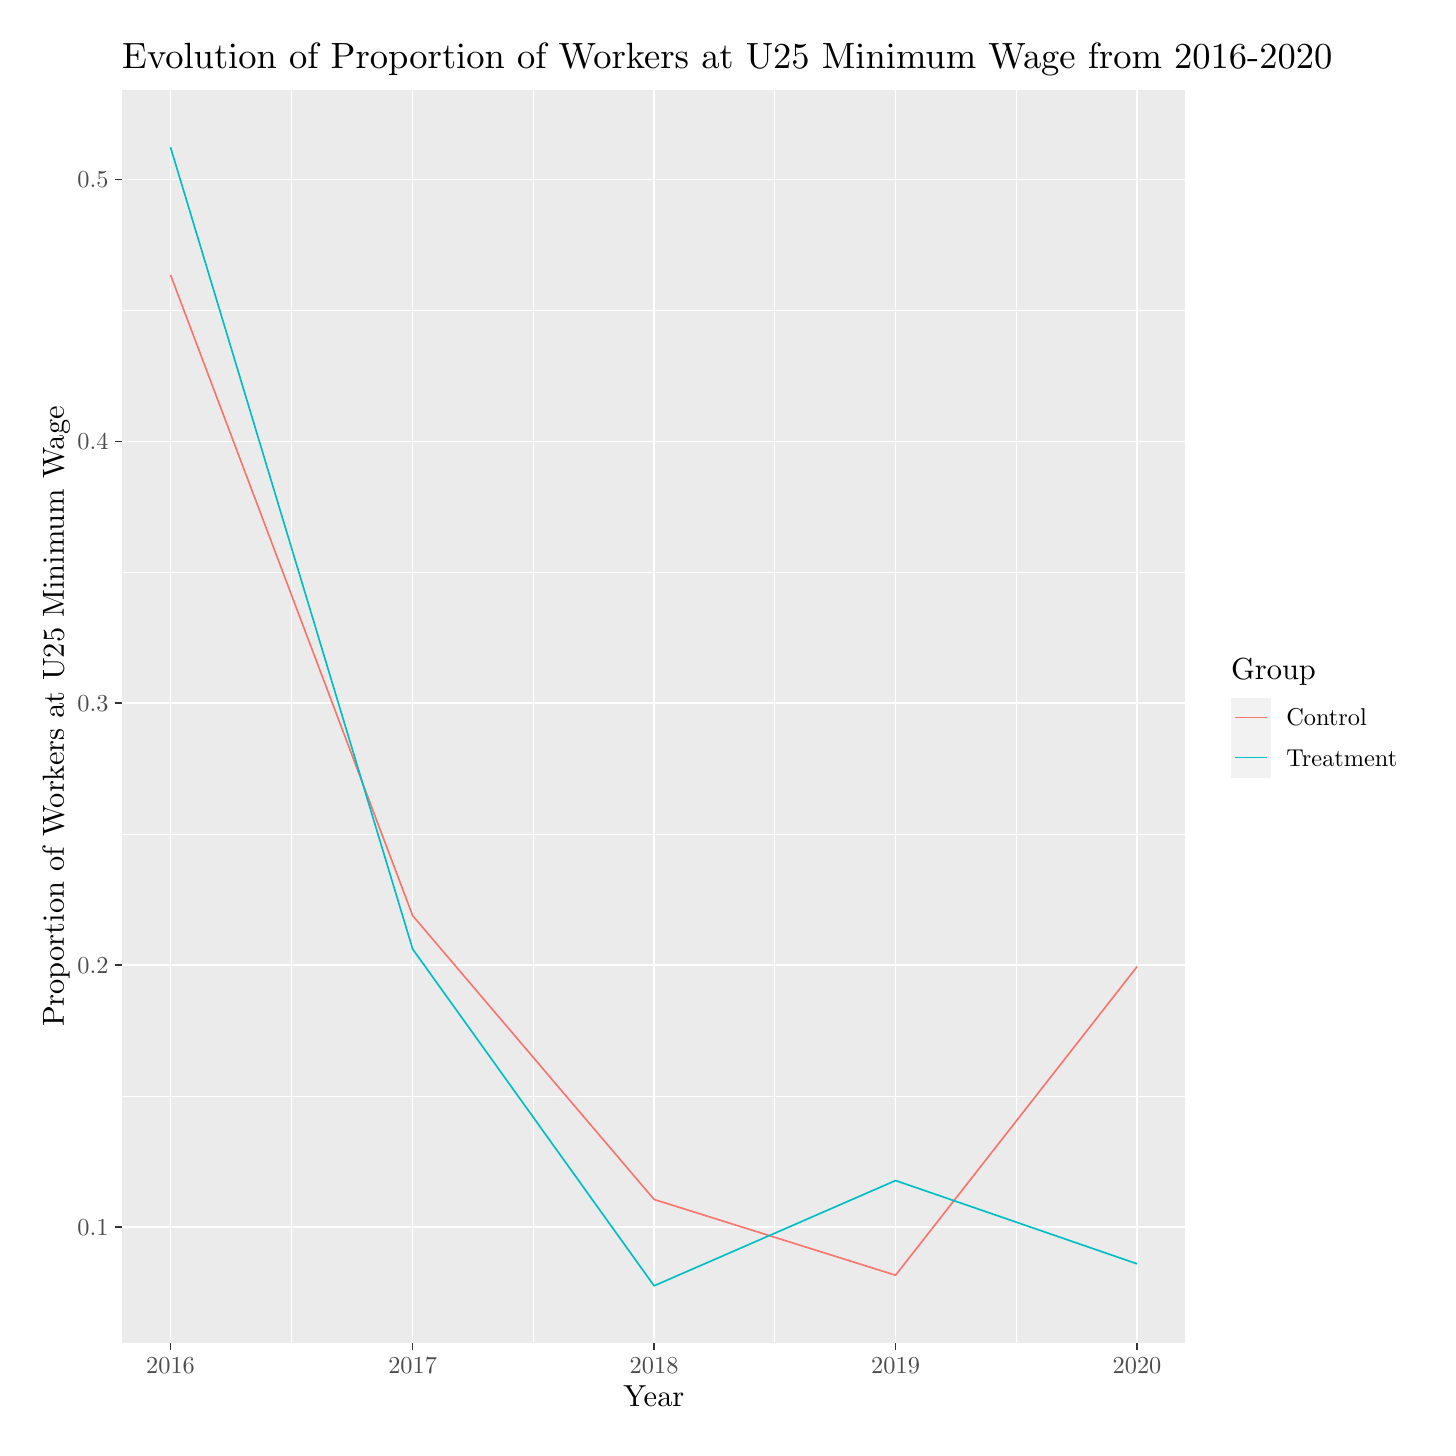
\begin{tikzpicture}[x=1pt,y=1pt]
\definecolor{fillColor}{RGB}{255,255,255}
\path[use as bounding box,fill=fillColor,fill opacity=0.00] (0,0) rectangle (505.89,505.89);
\begin{scope}
\path[clip] (  0.00,  0.00) rectangle (505.89,505.89);
\definecolor{drawColor}{RGB}{255,255,255}
\definecolor{fillColor}{RGB}{255,255,255}

\path[draw=drawColor,line width= 0.6pt,line join=round,line cap=round,fill=fillColor] (  0.00,  0.00) rectangle (505.89,505.89);
\end{scope}
\begin{scope}
\path[clip] ( 34.16, 30.69) rectangle (418.33,483.23);
\definecolor{fillColor}{gray}{0.92}

\path[fill=fillColor] ( 34.16, 30.69) rectangle (418.33,483.23);
\definecolor{drawColor}{RGB}{255,255,255}

\path[draw=drawColor,line width= 0.3pt,line join=round] ( 34.16,119.84) --
	(418.33,119.84);

\path[draw=drawColor,line width= 0.3pt,line join=round] ( 34.16,214.46) --
	(418.33,214.46);

\path[draw=drawColor,line width= 0.3pt,line join=round] ( 34.16,309.08) --
	(418.33,309.08);

\path[draw=drawColor,line width= 0.3pt,line join=round] ( 34.16,403.70) --
	(418.33,403.70);

\path[draw=drawColor,line width= 0.3pt,line join=round] ( 95.36, 30.69) --
	( 95.36,483.23);

\path[draw=drawColor,line width= 0.3pt,line join=round] (182.74, 30.69) --
	(182.74,483.23);

\path[draw=drawColor,line width= 0.3pt,line join=round] (269.99, 30.69) --
	(269.99,483.23);

\path[draw=drawColor,line width= 0.3pt,line join=round] (357.24, 30.69) --
	(357.24,483.23);

\path[draw=drawColor,line width= 0.6pt,line join=round] ( 34.16, 72.54) --
	(418.33, 72.54);

\path[draw=drawColor,line width= 0.6pt,line join=round] ( 34.16,167.15) --
	(418.33,167.15);

\path[draw=drawColor,line width= 0.6pt,line join=round] ( 34.16,261.77) --
	(418.33,261.77);

\path[draw=drawColor,line width= 0.6pt,line join=round] ( 34.16,356.39) --
	(418.33,356.39);

\path[draw=drawColor,line width= 0.6pt,line join=round] ( 34.16,451.00) --
	(418.33,451.00);

\path[draw=drawColor,line width= 0.6pt,line join=round] ( 51.62, 30.69) --
	( 51.62,483.23);

\path[draw=drawColor,line width= 0.6pt,line join=round] (139.11, 30.69) --
	(139.11,483.23);

\path[draw=drawColor,line width= 0.6pt,line join=round] (226.36, 30.69) --
	(226.36,483.23);

\path[draw=drawColor,line width= 0.6pt,line join=round] (313.62, 30.69) --
	(313.62,483.23);

\path[draw=drawColor,line width= 0.6pt,line join=round] (400.87, 30.69) --
	(400.87,483.23);
\definecolor{drawColor}{RGB}{248,118,109}

\path[draw=drawColor,line width= 0.6pt,line join=round] ( 51.62,416.54) --
	(139.11,185.03) --
	(226.36, 82.46) --
	(313.62, 55.09) --
	(400.87,166.58);
\definecolor{drawColor}{RGB}{0,191,196}

\path[draw=drawColor,line width= 0.6pt,line join=round] ( 51.62,462.66) --
	(139.11,172.95) --
	(226.36, 51.26) --
	(313.62, 89.30) --
	(400.87, 59.21);
\end{scope}
\begin{scope}
\path[clip] (  0.00,  0.00) rectangle (505.89,505.89);
\definecolor{drawColor}{gray}{0.30}

\node[text=drawColor,anchor=base east,inner sep=0pt, outer sep=0pt, scale=  0.88] at ( 29.21, 69.51) {0.1};

\node[text=drawColor,anchor=base east,inner sep=0pt, outer sep=0pt, scale=  0.88] at ( 29.21,164.12) {0.2};

\node[text=drawColor,anchor=base east,inner sep=0pt, outer sep=0pt, scale=  0.88] at ( 29.21,258.74) {0.3};

\node[text=drawColor,anchor=base east,inner sep=0pt, outer sep=0pt, scale=  0.88] at ( 29.21,353.36) {0.4};

\node[text=drawColor,anchor=base east,inner sep=0pt, outer sep=0pt, scale=  0.88] at ( 29.21,447.97) {0.5};
\end{scope}
\begin{scope}
\path[clip] (  0.00,  0.00) rectangle (505.89,505.89);
\definecolor{drawColor}{gray}{0.20}

\path[draw=drawColor,line width= 0.6pt,line join=round] ( 31.41, 72.54) --
	( 34.16, 72.54);

\path[draw=drawColor,line width= 0.6pt,line join=round] ( 31.41,167.15) --
	( 34.16,167.15);

\path[draw=drawColor,line width= 0.6pt,line join=round] ( 31.41,261.77) --
	( 34.16,261.77);

\path[draw=drawColor,line width= 0.6pt,line join=round] ( 31.41,356.39) --
	( 34.16,356.39);

\path[draw=drawColor,line width= 0.6pt,line join=round] ( 31.41,451.00) --
	( 34.16,451.00);
\end{scope}
\begin{scope}
\path[clip] (  0.00,  0.00) rectangle (505.89,505.89);
\definecolor{drawColor}{gray}{0.20}

\path[draw=drawColor,line width= 0.6pt,line join=round] ( 51.62, 27.94) --
	( 51.62, 30.69);

\path[draw=drawColor,line width= 0.6pt,line join=round] (139.11, 27.94) --
	(139.11, 30.69);

\path[draw=drawColor,line width= 0.6pt,line join=round] (226.36, 27.94) --
	(226.36, 30.69);

\path[draw=drawColor,line width= 0.6pt,line join=round] (313.62, 27.94) --
	(313.62, 30.69);

\path[draw=drawColor,line width= 0.6pt,line join=round] (400.87, 27.94) --
	(400.87, 30.69);
\end{scope}
\begin{scope}
\path[clip] (  0.00,  0.00) rectangle (505.89,505.89);
\definecolor{drawColor}{gray}{0.30}

\node[text=drawColor,anchor=base,inner sep=0pt, outer sep=0pt, scale=  0.88] at ( 51.62, 19.68) {2016};

\node[text=drawColor,anchor=base,inner sep=0pt, outer sep=0pt, scale=  0.88] at (139.11, 19.68) {2017};

\node[text=drawColor,anchor=base,inner sep=0pt, outer sep=0pt, scale=  0.88] at (226.36, 19.68) {2018};

\node[text=drawColor,anchor=base,inner sep=0pt, outer sep=0pt, scale=  0.88] at (313.62, 19.68) {2019};

\node[text=drawColor,anchor=base,inner sep=0pt, outer sep=0pt, scale=  0.88] at (400.87, 19.68) {2020};
\end{scope}
\begin{scope}
\path[clip] (  0.00,  0.00) rectangle (505.89,505.89);
\definecolor{drawColor}{RGB}{0,0,0}

\node[text=drawColor,anchor=base,inner sep=0pt, outer sep=0pt, scale=  1.10] at (226.24,  7.64) {Year};
\end{scope}
\begin{scope}
\path[clip] (  0.00,  0.00) rectangle (505.89,505.89);
\definecolor{drawColor}{RGB}{0,0,0}

\node[text=drawColor,rotate= 90.00,anchor=base,inner sep=0pt, outer sep=0pt, scale=  1.10] at ( 13.08,256.96) {Proportion of Workers at U25 Minimum Wage};
\end{scope}
\begin{scope}
\path[clip] (  0.00,  0.00) rectangle (505.89,505.89);
\definecolor{fillColor}{RGB}{255,255,255}

\path[fill=fillColor] (429.33,229.40) rectangle (500.39,284.52);
\end{scope}
\begin{scope}
\path[clip] (  0.00,  0.00) rectangle (505.89,505.89);
\definecolor{drawColor}{RGB}{0,0,0}

\node[text=drawColor,anchor=base west,inner sep=0pt, outer sep=0pt, scale=  1.10] at (434.83,270.38) {Group};
\end{scope}
\begin{scope}
\path[clip] (  0.00,  0.00) rectangle (505.89,505.89);
\definecolor{fillColor}{gray}{0.95}

\path[fill=fillColor] (434.83,249.35) rectangle (449.29,263.81);
\end{scope}
\begin{scope}
\path[clip] (  0.00,  0.00) rectangle (505.89,505.89);
\definecolor{drawColor}{RGB}{248,118,109}

\path[draw=drawColor,line width= 0.6pt,line join=round] (436.28,256.58) -- (447.84,256.58);
\end{scope}
\begin{scope}
\path[clip] (  0.00,  0.00) rectangle (505.89,505.89);
\definecolor{fillColor}{gray}{0.95}

\path[fill=fillColor] (434.83,234.90) rectangle (449.29,249.35);
\end{scope}
\begin{scope}
\path[clip] (  0.00,  0.00) rectangle (505.89,505.89);
\definecolor{drawColor}{RGB}{0,191,196}

\path[draw=drawColor,line width= 0.6pt,line join=round] (436.28,242.13) -- (447.84,242.13);
\end{scope}
\begin{scope}
\path[clip] (  0.00,  0.00) rectangle (505.89,505.89);
\definecolor{drawColor}{RGB}{0,0,0}

\node[text=drawColor,anchor=base west,inner sep=0pt, outer sep=0pt, scale=  0.88] at (454.79,253.55) {Control};
\end{scope}
\begin{scope}
\path[clip] (  0.00,  0.00) rectangle (505.89,505.89);
\definecolor{drawColor}{RGB}{0,0,0}

\node[text=drawColor,anchor=base west,inner sep=0pt, outer sep=0pt, scale=  0.88] at (454.79,239.09) {Treatment};
\end{scope}
\begin{scope}
\path[clip] (  0.00,  0.00) rectangle (505.89,505.89);
\definecolor{drawColor}{RGB}{0,0,0}

\node[text=drawColor,anchor=base west,inner sep=0pt, outer sep=0pt, scale=  1.32] at ( 34.16,491.30) {Evolution of Proportion of Workers at U25 Minimum Wage from 2016-2020};
\end{scope}
\end{tikzpicture}
